\documentclass[review]{elsarticle}

\usepackage{lineno,hyperref}
\modulolinenumbers[5]

\journal{Advances in Water Resources}

%%%%%%%%%%%%%%%%%%%%%%%
%% Elsevier bibliography styles
%%%%%%%%%%%%%%%%%%%%%%%
%% To change the style, put a % in front of the second line of the current style and
%% remove the % from the second line of the style you would like to use.
%%%%%%%%%%%%%%%%%%%%%%%

%% Numbered
%\bibliographystyle{model1-num-names}

%% Numbered without titles
%\bibliographystyle{model1a-num-names}

%% Harvard
%\bibliographystyle{model2-names.bst}\biboptions{authoryear}

%% Vancouver numbered
%\usepackage{numcompress}\bibliographystyle{model3-num-names}

%% Vancouver name/year
%\usepackage{numcompress}\bibliographystyle{model4-names}\biboptions{authoryear}

%% APA style
%\bibliographystyle{model5-names}\biboptions{authoryear}

%% AMA style
%\usepackage{numcompress}\bibliographystyle{model6-num-names}

%% `Elsevier LaTeX' style
\bibliographystyle{elsarticle-num}
%%%%%%%%%%%%%%%%%%%%%%%

\begin{document}

\begin{frontmatter}

\title{ Segmentation and Classification of Porous Media X-ray Images using Convolutional Neural Networks}


%% Group authors per affiliation:
\author{Efim Lavrukhin}

\author[mysecondaryaddress]{Gerke Kirill\corref{mycorrespondingauthor}}
\cortext[Gerke]{Corresponding author}
\ead{cheshik@.com}

%% or include affiliations in footnotes:
\author[mymainaddress,mysecondaryaddress]{Sizonenko Timothey}

\author[mymainaddress,mysecondaryaddress]{Korost Dmitry}

\author[tritaryaddress]{Tarasenko Sergey}

\address[mymainaddress]{Moscow, Russia}
\address[mysecondaryaddress]{Some Street}
\address[tritaryaddress]{Independent Researcher}

\begin{abstract}
Write abtract of the paper
\end{abstract}

\begin{keyword}
porous medium \sep image processing \sep convolutional neural network \sep image segmentation \sep segmentation networks
\end{keyword}

\end{frontmatter}

\linenumbers

\section{Introduction}

\section{Background and previous works}

\section{Methodology}
\subsection{Image processing applications for porous medium analysis}
\subsection{Convolutional neural networks for segmentation: breif review and benefits}
\subsection{Classifiers}

\section{Experiments}

\subsection{Porous medium specs}

\subsection{U-net architecture and features}

Key features of U-net architecture:
\begin{itemize}
	\item Fully-convolutional 
	\item Encoder-decoder acrchitecture with skip-connections
	\item Max pooling layres for comression in encoder part
	\item Transposed convolutional layers + concatenation with skip-connected encoder feature map for uncompression in decoder part
	\item Convolutional layers only with 3x3 filters
\end{itemize}

\begin{figure}[h]
	\center{
		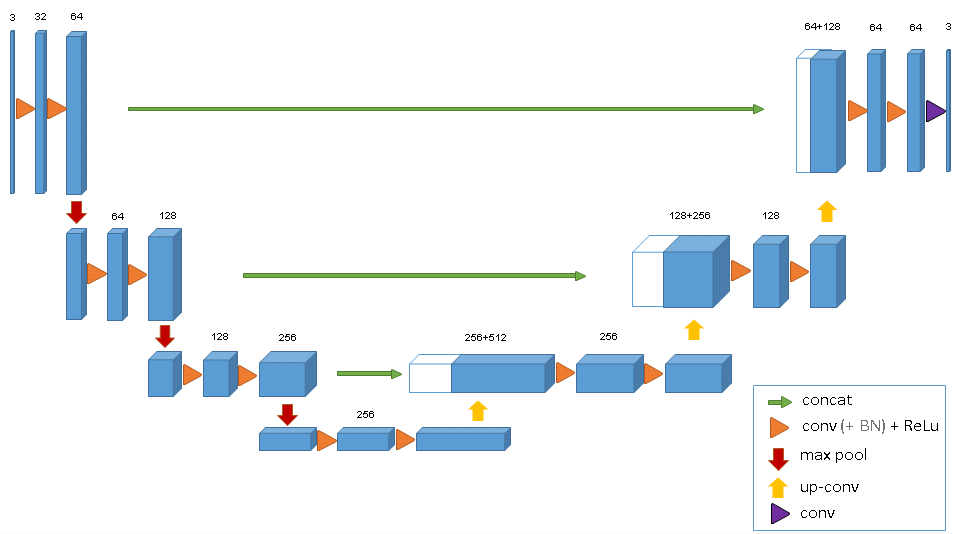
\includegraphics[width=1\linewidth]
			{data/Unet_architecture.png}
	}
	\caption{Unet architecture: ToDo}
	\label{Unet:architecture}
\end{figure}

We used Unet architecture  with some small features: 
\begin{itemize}
	\item Number of conv filters is multiplied by 32(insted of 64 in original article)
	\item Padding to conv filters, so network do not compress output
	\item ELU activation functions
	
\end{itemize}

\subsection{Specification of inputs into the neural network}

Our model get $700^3$ image stack as input. Than 2-d images splited into $64 \times 64$ patches with minimal overlapping, so our train data contains 84700 image patches($84700 \times 1 \times 64 \times 64$). Stack contains gray-scale images, so each image pixel's intensity scaled to $[-0.5, 0.5]$ interval. We do not use data augmentation because of data set size.

\begin{figure}[h]
	\center{
		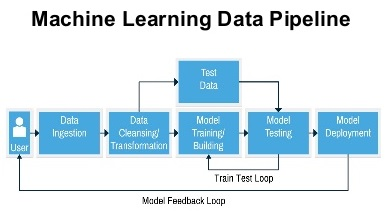
\includegraphics[width=1\linewidth]
			{data/data_pipeline.jpg}
	}
	\caption{Trainig pipeline: ToDo}
	\label{Unet:training}
\end{figure}

\subsection{Learning process}

We used combination of cross-entropy and smoothed IOU as loss function:
\begin{equation}{\label{Loss}}
	L(x, y) = \frac{1}{N} 
		\sum \limits_{i = 1}^{N} 
		\sum \limits_{x, y \in I_{i}, M_{i}} 
		\frac{1}{W H} \Bigl( 
		y \log p(x) 
		+ \alpha \log 
		\frac{p(x) y + \varepsilon}{p(x) + y - p(x)y + \varepsilon}
		\Bigr)
\end{equation}
with $\varepsilon=10^{-5}$.

We used Adam optimizer with initial learning rate $=10^{-3}$ and 
multiplicative learning rate decay to $10^{-5}$ until final epoch.

We choose size of minibatch equals $=32$ and train our model during 10 epochs. We used only $\frac{1}{5}$ randomly choosen part of training patches in each epoch.

\subsection{Experimantal set-up}
We choose 3 rock types: carbonate, soil and sanstone. We have 
4 carbonate, 4 soil and 3 sandstone stacks. We choose one of stacks from each category as trained(carbonate 1, soil 1 and sandstone 1).
Then we train 3 models on each trained stack independenlty, 3 models on each pair of trained stacks and one model on both trained stacks.
As result we have 7 models to compare.
We measure different metrics(logloss, IOU, accuracy, precision, recall, PR-AUC) with diffent thresholds on each of 11 stacks.


\section{Results}

\subsection{Classification with and without segmentaion}

\subsection{Classification of patterns from various media}

\section{Discussion}
Overview of results and applicability of the results.

\section{Conclusion}
General conclusion and future work.

\section*{References}

\bibliography{mybibfile}

\end{document}